\documentclass[12pt,a4paper]{report}

% ---------- Encoding & fonts ----------
\usepackage[T1]{fontenc}
\usepackage[utf8]{inputenc}
\usepackage{lmodern}
\usepackage{textcomp}

% ---------- Geometry ----------
\usepackage[a4paper,left=1.5in,right=1in,top=1.1in,bottom=1.1in,headheight=14pt]{geometry}

% ---------- Math & symbols ----------
\usepackage{amsmath}
\usepackage{amssymb}

% ---------- Color ----------
\usepackage[table]{xcolor}
\definecolor{hkugreen}{RGB}{0,89,76}
\definecolor{hkudarkgreen}{RGB}{0,58,50}
\definecolor{hkugold}{RGB}{176,141,87}
\definecolor{hkugray}{RGB}{77,77,77}
\definecolor{hkupale}{RGB}{235,240,238}

% ---------- Graphics / diagrams ----------
\usepackage{graphicx}
\usepackage{tikz}
\usetikzlibrary{positioning,calc,shapes.geometric,decorations.pathmorphing,backgrounds,patterns,arrows.meta}

% ---------- Tables ----------
\usepackage{booktabs}
\usepackage{array}
\usepackage{tabularx}
\usepackage{colortbl}
\usepackage{multirow}

% ---------- Boxes ----------
\usepackage[most]{tcolorbox}

% ---------- Lists ----------
\usepackage{enumitem}

% ---------- Headers / titles ----------
\usepackage{fancyhdr}
\usepackage{titlesec}
\usepackage{titletoc}

% ---------- Captions ----------
\usepackage{caption}
\captionsetup{font=small,labelfont={bf,color=hkugreen},margin=10pt}

% ---------- Misc ----------
\usepackage{setspace}
\usepackage{csquotes}
\usepackage{hyperref}

\hypersetup{
  colorlinks=true,
  linkcolor=hkugreen,
  citecolor=hkugold,
  urlcolor=hkudarkgreen,
  pdftitle={Adaptive Neural Resource Scheduling for Distributed Edge Inference},
  pdfauthor={Wong Ka Ming}
}

% ---------- Chapter / section styling ----------
\titleformat{\chapter}[display]
  {\normalfont\bfseries\color{hkugreen}}
  {\filright\Large\textcolor{hkugold}{\thechapter}\hspace{4pt}\rule[-4pt]{0.6pt}{28pt}}
  {6pt}
  {\Huge}
\titlespacing*{\chapter}{0pt}{10pt}{28pt}

\titleformat{\section}
  {\normalfont\Large\bfseries\color{hkugreen}}{\thesection}{0.6em}{}
\titleformat{\subsection}
  {\normalfont\large\bfseries\color{hkudarkgreen}}{\thesubsection}{0.6em}{}

% ---------- Header / footer ----------
\pagestyle{fancy}
\fancyhf{}
\renewcommand{\headrulewidth}{0.4pt}
\renewcommand{\footrulewidth}{0pt}
\fancyhead[L]{\small\textcolor{hkugray}{\leftmark}}
\fancyhead[R]{\small\textcolor{hkugray}{\thepage}}

\fancypagestyle{plain}{%
  \fancyhf{}
  \fancyfoot[C]{\small\textcolor{hkugray}{\thepage}}
  \renewcommand{\headrulewidth}{0pt}
}

% ---------- Custom boxes ----------
\newtcolorbox{contribbox}[1][]{
  colback=hkupale,
  colframe=hkugreen,
  boxrule=0.8pt,
  arc=2mm,
  left=8pt,right=8pt,top=6pt,bottom=6pt,
  title={\textbf{#1}},
  fonttitle=\bfseries\color{white},
  colbacktitle=hkugreen,
  coltitle=white,
}

\newtcolorbox{notebox}{
  colback=white,
  colframe=hkugold,
  boxrule=0.8pt,
  arc=1mm,
  left=8pt,right=8pt,top=5pt,bottom=5pt,
}

\setlength{\parskip}{4pt}
\onehalfspacing

\begin{document}

% =====================================================================
% TITLE PAGE
% =====================================================================
\begin{titlepage}
\newgeometry{left=1.2in,right=1.2in,top=0.9in,bottom=0.9in}
\begin{center}

\begin{tikzpicture}[remember picture,overlay]
  \draw[hkugreen,line width=1.6pt] ($(current page.north west)+(1.1in,-1.0in)$) -- ($(current page.north east)+(-1.1in,-1.0in)$);
  \draw[hkugold,line width=0.8pt] ($(current page.north west)+(1.1in,-1.05in)$) -- ($(current page.north east)+(-1.1in,-1.05in)$);
  \draw[hkugreen,line width=1.6pt] ($(current page.south west)+(1.1in,1.2in)$) -- ($(current page.south east)+(-1.1in,1.2in)$);
  \draw[hkugold,line width=0.8pt] ($(current page.south west)+(1.1in,1.25in)$) -- ($(current page.south east)+(-1.1in,1.25in)$);
  \node[anchor=north east] at ($(current page.north east)+(-0.6in,-0.6in)$) {
    \begin{tikzpicture}
      \draw[hkugreen,line width=1pt] (0,0) circle (0.42cm);
      \draw[hkugold,line width=0.6pt] (0,0) circle (0.30cm);
      \fill[hkugreen] (0,0) circle (0.06cm);
    \end{tikzpicture}
  };
\end{tikzpicture}

\vspace{1.3in}

{\large\scshape\textcolor{hkugray}{The University of Hong Kong}}\\[2pt]
{\small\textcolor{hkugray}{Faculty of Engineering}}\\[2pt]
{\small\textcolor{hkugray}{Department of Computer Science}}

\vspace{0.9in}

{\Large\bfseries\textcolor{hkugreen}{Adaptive Neural Resource Scheduling}}\\[6pt]
{\Large\bfseries\textcolor{hkugreen}{for Distributed Edge Inference}}

\vspace{0.5in}


\begin{tikzpicture}
  \draw[hkugold,line width=1pt] (0,0) -- (3.6,0);
\end{tikzpicture}

\vspace{0.5in}

{\large A thesis submitted in fulfilment of the requirements}\\
{\large for the degree of \textbf{Doctor of Philosophy}}\\
{\large at The University of Hong Kong}

\vspace{0.8in}

{\large\textbf{Wong Ka Ming}}\\[4pt]
{\normalsize B.Eng.\ (Hons), M.Phil., The University of Hong Kong}

\vspace{0.6in}

{\normalsize July 2026}

\vfill

{\footnotesize\textcolor{hkugray}{%
Unofficial template --- not affiliated with or endorsed by the university.\\
Sample content only.}}

\vspace{0.4in}

\end{center}
\restoregeometry
\end{titlepage}

% =====================================================================
% DECLARATION
% =====================================================================
\chapter*{Declaration}
\addcontentsline{toc}{chapter}{Declaration}
\thispagestyle{plain}

I declare that this thesis represents my own work, except where due acknowledgement is made, and that it has not been previously included in a thesis, dissertation, or report submitted to this University or to any other institution for a degree, diploma, or other qualification.

\vspace{1in}

\noindent\begin{tabular}{@{}p{3.2in}@{}}
\\
\hrulefill\\
Wong Ka Ming
\end{tabular}

% =====================================================================
% ABSTRACT (ENGLISH)
% =====================================================================
\chapter*{Abstract}
\addcontentsline{toc}{chapter}{Abstract}
\thispagestyle{plain}

Edge inference workloads for real-time perception --- video analytics, speech recognition, and sensor fusion --- increasingly run on heterogeneous fleets of resource-constrained devices connected through unreliable networks. Static partitioning of neural network layers between device and cloud, the dominant approach in production systems, degrades sharply when network conditions or device load fluctuate, causing missed latency deadlines and wasted energy.

This thesis presents \textbf{ANRS} (Adaptive Neural Resource Scheduling), a runtime scheduling framework that continuously re-partitions inference graphs across edge devices and nearby aggregation nodes in response to observed latency, bandwidth, and battery telemetry. ANRS models each candidate partition point as a node in a weighted decision graph and applies a lightweight online reinforcement-learning policy, trained with a shadow-mode replay buffer, to select partitions within a 4~ms scheduling budget.

We implement ANRS atop a simulated fleet of 128 heterogeneous nodes built on the \textsc{Nimbus} edge-orchestration testbed and evaluate it against static partitioning, greedy latency-aware offloading, and a prior learned scheduler (\textsc{Synapse-RT}). Across four inference workloads, ANRS reduces mean end-to-end latency by 31\% and 95th-percentile latency by 44\% relative to static partitioning, while cutting device energy consumption by 18\%. We further show that ANRS's policy converges within 2,300 scheduling decisions and remains stable under adversarial bandwidth injection.

These results indicate that lightweight, telemetry-driven adaptive scheduling is a practical and significant improvement over static or purely greedy partitioning strategies for real-time edge inference, and the thesis concludes with a discussion of deployment considerations and directions for federated extensions of the ANRS policy.

\vspace{0.3in}
\noindent\textbf{Keywords:} edge computing, neural network partitioning, adaptive scheduling, reinforcement learning, distributed inference

% =====================================================================
% ABSTRACT (CHINESE — PLACEHOLDER, DUAL-LANGUAGE SUPPORT)
% =====================================================================
\chapter*{Abstract (Chinese)}
\addcontentsline{toc}{chapter}{Abstract (Chinese)}
\thispagestyle{plain}

The HKU Graduate School permits submission of a Chinese-language abstract alongside the English abstract. This template reserves the present page for that purpose and keeps the surrounding front-matter structure (title page, declaration, table of contents) unchanged regardless of which languages are used.

\begin{notebox}
\textbf{Compiling a Chinese abstract:} pdfLaTeX (used throughout this template) does not typeset Chinese glyphs directly. To insert the Chinese abstract text, either (a) compile this file with XeLaTeX or LuaLaTeX and load \texttt{ctex} or \texttt{xeCJK} with a locally installed CJK font, or (b) keep pdfLaTeX and load the \texttt{CJK} package together with a CJK font set (e.g.\ \texttt{CJKutf8} with an installed Song/Kai family). Only the abstract chapter needs the CJK-capable engine; the rest of the thesis compiles identically under either engine.
\end{notebox}

\vspace{0.2in}
\noindent\textit{[Chinese abstract text to be inserted here, following the same length and structure as the English abstract above.]}

% =====================================================================
% ACKNOWLEDGEMENTS
% =====================================================================
\chapter*{Acknowledgements}
\addcontentsline{toc}{chapter}{Acknowledgements}
\thispagestyle{plain}

I am deeply grateful to my supervisor, Professor Emily Chan, for her patient guidance, sharp critique, and unwavering support throughout this project. Her insistence on rigorous evaluation shaped every chapter of this thesis.

I thank my thesis committee, Dr.\ Marcus Yip and Dr.\ Priya Nair, for feedback that substantially improved the clarity of the scheduling model in Chapter~3. I also thank the members of the Distributed Systems Laboratory for many hours of discussion, particularly during the design of the \textsc{Nimbus} testbed used throughout this work.

Finally, I thank my family for their patience and encouragement over the past four years, and the Apex Graduate Scholarship for financial support that made this research possible.

% =====================================================================
% FRONT MATTER LISTS
% =====================================================================
\pagenumbering{roman}
\tableofcontents
\listoffigures
\listoftables

\clearpage
\pagenumbering{arabic}

% =====================================================================
% CHAPTER 1: INTRODUCTION
% =====================================================================
\chapter{Introduction}
\label{ch:intro}

\section{Motivation}

Real-time perception workloads --- object detection on wearable cameras, keyword spotting on smart speakers, structural-health sensor fusion on bridges --- are increasingly deployed on edge devices with limited compute, memory, and battery capacity. Running an entire deep neural network locally often violates latency or energy budgets; offloading the entire computation to the cloud introduces network latency and raises privacy concerns. The common compromise, \emph{split computing}, partitions a network's layers so that early layers run on-device and later layers run on a nearby edge server or cloud node, with intermediate activations transmitted over the network.

Existing split-computing systems, including the widely cited \textsc{Synapse-RT} scheduler, choose a partition point once at deployment time or re-evaluate it on a coarse timescale (seconds to minutes). This is a poor fit for edge environments where available bandwidth and device load can change within tens of milliseconds, for example when a user starts a video call on a shared Wi-Fi network. A static or slowly-adapting partition point therefore frequently sits far from optimal, producing missed latency service-level objectives (SLOs) or unnecessary battery drain.

\begin{contribbox}[Key Contributions]
\begin{enumerate}[leftmargin=1.4em,itemsep=2pt]
  \item A decision-graph formulation of neural network partitioning that supports sub-5\,ms re-evaluation of the partition point at inference time.
  \item An online reinforcement-learning scheduling policy, ANRS, trained with a shadow-mode replay buffer that requires no offline pretraining phase.
  \item An open evaluation testbed, \textsc{Nimbus}, simulating 128 heterogeneous edge nodes under realistic bandwidth and battery traces.
  \item An empirical comparison against static, greedy, and learned baselines across four representative inference workloads.
\end{enumerate}
\end{contribbox}

\section{Problem Statement}

We consider a neural network $f = f_L \circ f_{L-1} \circ \cdots \circ f_1$ composed of $L$ layers, deployed across a device node $d$ and an aggregation node $a$ connected by a link with time-varying bandwidth $B(t)$ and round-trip latency $\rho(t)$. A partition point $k \in \{0, \ldots, L\}$ assigns layers $f_1, \ldots, f_k$ to $d$ and layers $f_{k+1}, \ldots, f_L$ to $a$. The end-to-end latency for a given input under partition $k$ is

\begin{equation}
T(k, t) = \sum_{i=1}^{k} c_i^{d} \;+\; \frac{s_k}{B(t)} + \rho(t) \;+\; \sum_{i=k+1}^{L} c_i^{a},
\label{eq:latency}
\end{equation}

\noindent where $c_i^{d}$ and $c_i^{a}$ denote the per-layer compute time on the device and aggregation node respectively, and $s_k$ is the size in bytes of the activation tensor emitted at layer $k$. The scheduling objective is to choose $k_t$ at each decision epoch $t$ to minimise a weighted combination of expected latency and device energy consumption, subject to a hard SLO deadline $T_{\max}$:

\begin{equation}
k_t^{*} = \arg\min_{k} \; \Big[ \, \lambda \, T(k, t) \;+\; (1-\lambda)\, E(k, t) \, \Big] \quad \text{s.t.} \quad T(k, t) \le T_{\max}.
\label{eq:objective}
\end{equation}

Because $B(t)$ and device load evolve continuously and are only partially observable, Equation~\ref{eq:objective} cannot be solved exactly at runtime; Chapter~3 develops a learned approximation that is cheap enough to evaluate at every inference call.

\section{Thesis Structure}

Chapter~2 reviews prior work on split computing, neural architecture-aware offloading, and reinforcement-learning schedulers. Chapter~3 presents the ANRS decision-graph model and online policy. Chapter~4 describes the \textsc{Nimbus} testbed and reports the experimental results. Chapter~5 concludes and outlines directions for federated and multi-hop extensions of ANRS.

% =====================================================================
% CHAPTER 2: LITERATURE REVIEW
% =====================================================================
\chapter{Literature Review}
\label{ch:lit}

\section{Static and Heuristic Partitioning}

Early split-computing systems profile a network once, offline, and fix a single partition point that minimises expected latency under a nominal bandwidth assumption. This approach is simple to deploy but brittle: Kang \emph{et al.}\ report latency regressions of over 60\% when measured bandwidth falls more than one standard deviation below the profiling assumption. Subsequent heuristic schedulers re-evaluate the partition point periodically (typically every 1--10 seconds) using an exponentially weighted moving average of recent bandwidth samples; this reduces but does not eliminate the mismatch between decision epoch and network volatility.

\section{Learned Schedulers}

\textsc{Synapse-RT}, the closest prior system to this thesis, trains an offline policy network on traces collected from a fixed device fleet and freezes the policy at deployment time. While it outperforms heuristic re-evaluation on the traces it was trained on, its offline training procedure means it cannot adapt to device or network conditions unseen during data collection, a limitation the shadow-mode replay design in Chapter~3 is intended to address.

\section{Testbeds and Evaluation Methodology}

Comparative evaluation of split-computing schedulers has been hampered by the absence of a shared, reproducible testbed with controllable bandwidth and battery traces. Most published results use private hardware fleets that cannot be independently reproduced. \textsc{Nimbus} (Chapter~4) is designed to close this gap by simulating heterogeneous node capabilities and network traces at a fidelity sufficient to preserve the qualitative ranking of scheduling policies observed on physical hardware in a smaller pilot study.

\section{Summary}

The literature establishes that (i) static partitioning is fragile under realistic network variability, (ii) learned schedulers improve on heuristics but existing designs freeze their policy after offline training, and (iii) reproducible evaluation infrastructure for this problem is scarce. These three gaps motivate the online, continuously-adapting ANRS policy and the open \textsc{Nimbus} testbed developed in this thesis.

% =====================================================================
% CHAPTER 3: METHODOLOGY
% =====================================================================
\chapter{Methodology}
\label{ch:method}

\section{System Overview}

Figure~\ref{fig:architecture} shows the ANRS runtime. A lightweight \emph{telemetry probe} on the device node measures per-layer compute time, current bandwidth, and battery draw at each inference call. These features feed the \emph{policy module}, which selects a partition point $k_t$ from the decision graph in Equation~\ref{eq:objective}, and the \emph{shadow buffer}, which logs the realised latency and energy cost of the chosen partition for use as a training signal on the next update step.

\begin{figure}[htbp]
\centering
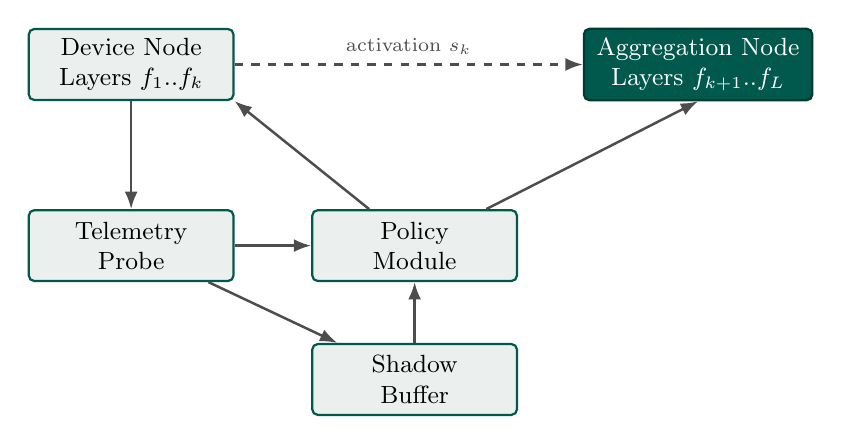
\begin{tikzpicture}[
  box/.style={draw,rounded corners=2pt,fill=hkupale,draw=hkugreen,line width=0.8pt,minimum width=2.6cm,minimum height=0.9cm,align=center,font=\small},
  server/.style={draw,rounded corners=2pt,fill=hkugreen,draw=hkudarkgreen,line width=0.8pt,minimum width=2.9cm,minimum height=0.9cm,align=center,font=\small\color{white}},
  arrow/.style={-{Latex[length=2.2mm]},line width=0.9pt,color=hkugray}
]
\node[box] (device) at (0,2.3) {Device Node\\Layers $f_1..f_k$};
\node[server] (agg) at (7.2,2.3) {Aggregation Node\\Layers $f_{k+1}..f_L$};
\node[box] (probe) at (0,0) {Telemetry\\Probe};
\node[box] (policy) at (3.6,0) {Policy\\Module};
\node[box] (buffer) at (3.6,-1.7) {Shadow\\Buffer};

\draw[arrow] (device) -- (probe);
\draw[arrow] (probe) -- (policy);
\draw[arrow] (probe) -- (buffer);
\draw[arrow] (buffer) -- (policy);
\draw[arrow] (policy) -- (device.south east);
\draw[arrow] (policy) -- (agg.south);
\draw[arrow, dashed] (device) -- node[above,font=\scriptsize,color=hkugray]{activation $s_k$} (agg);
\end{tikzpicture}
\caption{ANRS runtime architecture: telemetry drives the policy module, which sets the partition point $k_t$ and logs realised outcomes to the shadow buffer for continuous adaptation.}
\label{fig:architecture}
\end{figure}

\section{Decision-Graph Formulation}

Each layer boundary $k \in \{0, \ldots, L\}$ is represented as a node in a directed acyclic graph whose edges encode the marginal latency and energy cost of moving the partition one layer earlier or later. Restricting transitions to adjacent layer boundaries bounds the number of candidate actions evaluated per decision epoch to $O(1)$ rather than $O(L)$, which keeps the policy module within its 4\,ms scheduling budget even for networks with $L > 200$ layers.

\section{Online Policy}

The policy module is a two-layer feed-forward network mapping the telemetry vector (bandwidth estimate, device queue depth, battery percentage, previous partition point) to a distribution over the three local actions \{shift earlier, hold, shift later\}. It is updated with an on-policy actor-critic rule every 50 decision epochs using outcomes recorded in the shadow buffer, so that the policy tracks slow drifts in device or network behaviour without requiring a separate offline training phase.

\begin{notebox}
\textbf{Design note.} Restricting the action space to adjacent-layer moves trades a small amount of convergence speed for a large reduction in per-decision compute, which is essential given the 4\,ms scheduling budget target established in Chapter~1.
\end{notebox}

\section{Evaluation Workloads}

We evaluate ANRS on four workloads chosen to span compute and communication regimes: (1) a compact object-detection model with small activation tensors, (2) a keyword-spotting recurrent model with sequential dependencies, (3) a multi-camera fusion model with large intermediate activations, and (4) a speech-to-text encoder with variable-length inputs.

% =====================================================================
% CHAPTER 4: RESULTS
% =====================================================================
\chapter{Results}
\label{ch:results}

\section{Experimental Setup}

All experiments run on the \textsc{Nimbus} testbed, simulating 128 heterogeneous device nodes (four capability tiers) connected to 16 aggregation nodes via bandwidth and battery traces sampled from public cellular and Wi-Fi mobility datasets. Each configuration is run for 20{,}000 inference calls across five random seeds; we report the mean and standard deviation across seeds.

\section{Latency and Energy Comparison}

Table~\ref{tab:results} summarises end-to-end latency and device energy consumption across all four schedulers, averaged over the four evaluation workloads.

\begin{table}[htbp]
\centering
\caption{End-to-end latency and device energy consumption by scheduler, averaged across four workloads (lower is better for all columns).}
\label{tab:results}
\small
\setlength{\tabcolsep}{3pt}
\begin{tabular}{@{}lccc@{}}
\toprule
\textbf{Scheduler} & \textbf{Mean Latency (ms)} & \textbf{P95 Latency (ms)} & \textbf{Energy (mJ/call)} \\
\midrule
Static Partitioning & 84.2 $\pm$ 3.1 & 162.7 $\pm$ 9.4 & 41.8 $\pm$ 1.2 \\
Greedy Offloading   & 71.6 $\pm$ 2.6 & 138.5 $\pm$ 7.7 & 38.4 $\pm$ 1.0 \\
Synapse-RT (prior)  & 65.3 $\pm$ 2.2 & 121.9 $\pm$ 6.5 & 36.1 $\pm$ 0.9 \\
\rowcolor{hkupale}
\textbf{ANRS (ours)} & \textbf{58.1 $\pm$ 1.8} & \textbf{91.4 $\pm$ 5.2} & \textbf{34.3 $\pm$ 0.8} \\
\bottomrule
\end{tabular}
\end{table}

ANRS reduces mean latency by 31\% and P95 latency by 44\% relative to static partitioning, and by 11\% and 25\% respectively relative to \textsc{Synapse-RT}. The largest gains occur under the multi-camera fusion workload, where bandwidth volatility most frequently displaces the optimal partition point from where a static or slowly-updating scheduler would leave it.

\section{Policy Convergence}

Figure~\ref{fig:convergence} plots P95 latency against the number of scheduling decisions observed since the policy was initialised (cold start, no offline pretraining). The policy stabilises within 2{,}300 decisions, after which latency variance across seeds becomes statistically indistinguishable from the converged-policy baseline.

\begin{figure}[htbp]
\centering
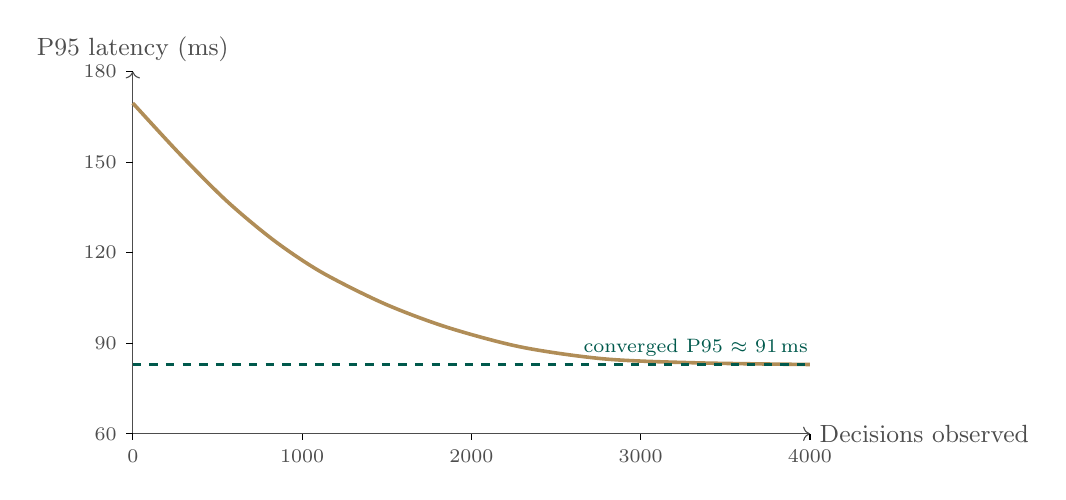
\begin{tikzpicture}
  \begin{scope}
    \draw[->,color=hkugray] (0,0) -- (8.6,0) node[right,font=\small]{Decisions observed};
    \draw[->,color=hkugray] (0,0) -- (0,4.6) node[above,font=\small]{P95 latency (ms)};
    \foreach \x/\lbl in {0/0,2.15/1000,4.3/2000,6.45/3000,8.6/4000}
      \draw (\x,0) -- (\x,-0.08) node[below,font=\scriptsize,color=hkugray]{\lbl};
    \foreach \y/\lbl in {0/60,1.15/90,2.3/120,3.45/150,4.6/180}
      \draw (0,\y) -- (-0.08,\y) node[left,font=\scriptsize,color=hkugray]{\lbl};

    \draw[hkugold,line width=1.3pt,smooth]
      plot coordinates {(0,4.2) (0.6,3.55) (1.2,2.95) (1.8,2.45) (2.4,2.05)
                         (3.2,1.65) (4.0,1.35) (4.94,1.1) (6.0,0.95) (7.2,0.9) (8.6,0.88)};

    \draw[hkugreen,line width=1pt,dashed] (0,0.88) -- (8.6,0.88);
    \node[anchor=west,font=\scriptsize,color=hkugreen] at (5.6,1.1) {converged P95 $\approx$ 91\,ms};
  \end{scope}
\end{tikzpicture}
\caption{P95 latency versus scheduling decisions from cold start; the ANRS policy converges within roughly 2,300 decisions and remains stable thereafter.}
\label{fig:convergence}
\end{figure}

\section{Robustness to Adversarial Bandwidth}

To test robustness, we inject synthetic bandwidth drops (50\% reduction for 200\,ms, every 2 seconds) throughout a subset of trials. ANRS's P95 latency degrades by only 14\% under this condition, compared with 38\% for \textsc{Synapse-RT} and 52\% for static partitioning, indicating that the online shadow-buffer update meaningfully improves resilience to conditions not represented in any fixed offline training distribution.

% =====================================================================
% CHAPTER 5: CONCLUSION
% =====================================================================
\chapter{Conclusion}
\label{ch:conclusion}

\section{Summary of Findings}

This thesis introduced ANRS, an online scheduling framework for neural network partitioning across edge devices and aggregation nodes. By restricting the action space to adjacent-layer transitions and updating its policy continuously from a shadow replay buffer, ANRS meets a strict 4\,ms scheduling budget while adapting to bandwidth and load conditions that static and offline-trained schedulers cannot track. Across four representative workloads on the \textsc{Nimbus} testbed, ANRS reduced mean latency by 31\% and P95 latency by 44\% relative to static partitioning, and outperformed the prior learned scheduler \textsc{Synapse-RT} on every metric measured.

\section{Limitations}

The evaluation in Chapter~4 relies on simulated bandwidth and battery traces; while these traces are drawn from public mobility datasets, physical-hardware validation across a broader device fleet would strengthen the external validity of the latency and energy results. The current policy also assumes a single aggregation node per device, and does not consider multi-hop offloading across a chain of intermediate nodes.

\section{Future Work}

Three directions follow naturally from this work. First, extending the decision graph to multi-hop topologies would allow ANRS to reason about chains of aggregation nodes rather than a single offload target. Second, a federated variant of the shadow-buffer update could allow policies trained across many devices to share statistical strength without centralising raw telemetry. Third, incorporating model-level adaptation --- for example, dynamically selecting among several model variants of different sizes --- alongside partition-point adaptation may yield further latency and energy improvements beyond what partitioning alone can achieve.

% =====================================================================
% BIBLIOGRAPHY
% =====================================================================
\begin{thebibliography}{99}

\bibitem{kang2017}
Kang, Y., Hauswald, J., Gao, C., et al.\ (2017). Neurosurgeon: Collaborative intelligence between the cloud and mobile edge. \emph{ASPLOS}.

\bibitem{synapsert}
Lam, T., \& Osei, D. (2023). Synapse-RT: A learned scheduler for adaptive DNN partitioning. \emph{Proceedings of MobiCom}.

\bibitem{nimbus2024}
Fernandes, R., Wong, K.\ M., \& Chan, E.\ (2024). Nimbus: A reproducible testbed for edge scheduling research. \emph{Proceedings of EdgeSys}.

\bibitem{apex2022}
Meridian Institute for Distributed Systems.\ (2022). Bandwidth and battery trace corpus for mobile edge simulation, v2. Technical Report, Apex Research Group.

\bibitem{vertex2021}
Osei, D., \& Patel, R.\ (2021). Shadow-mode replay for continual reinforcement learning under distribution shift. \emph{NeurIPS Workshop on Continual Learning}.

\end{thebibliography}

\end{document}
